%================================================================
%                   HELMHOLTZ EQUATION
%
%                 last reviewed on 28/04
%================================================================
\section{The Helmholtz equation}
Up to this point we have been thinking of the velocity field as a function of three dimensional space $(x, y, z)$ and time $t$. As it stands finding an expression for this velocity field could get very complex because of the amount of variables we'd have to juggle. A classical way to deal with is is to separate the problem into two: a time-dependent, and a time-independent problem.

To do this, employ a standard separation of variables argument. We propose that, since $\phi(\vec{x}, t)$, there exist $X$ and $T$ such that
  \begin{equation}\label{eq:phi_separation}
      \phi = X(\vec{x})T(t).
  \end{equation}

We still require that $\vec{u}$ satisfies the linear wave equation. From proposition \ref{propn:potential_satisfies_linear_wave_eq} we know that this is equivalent to $\phi$ satisfying the linear wave equation. Hence we have
  \begin{align*}
      T(t) \nabla^2 X(\vec{x})
      &= \frac{1}{c^2} \frac{d^2 T}{dt^2} X(\vec{x}), \\
      \frac{\nabla^2 X}{X} &= \frac{1}{c^2} \frac{\ddot{T}}{T}.
  \end{align*}

This can only be true if both sides are equal to the same constant, say $\ell^2 \in \bb{C}$. We therefore yield two ordinary differential equations:
    \begin{multicols}{2}
    \noindent
        \begin{equation} \label{eq:helmholtz_eigenvalue}
            \nabla^2 X = \ell^2 X,
        \end{equation}
        \begin{equation}\label{eq:helmholtz_time_dep}
            \ddot{T} - \ell^2 c^2 T = 0.
        \end{equation}
    \end{multicols}\par
%
Equation \eqref{eq:helmholtz_eigenvalue} represents a time independent form of the linear wave equation, the Helmholtz equation, \eqref{eq:helmholtz_time_dep} can be solved to find an expression for the the time dependence of the velocity field.

Equation \eqref{eq:helmholtz_time_dep} is a second order linear homogeneous ordinary differential equation with constant coefficients. The general solution for this type of equation is
\begin{align}\label{eq:gen_sol_time_dep}
  T(t) = e^{\omega_1t} + e^{-\omega_2t}.
\end{align}

Inputting this into \ref{eq:helmholtz_time_dep},
\begin{gather*}
  \omega_1^2e^{\omega_1t} + \omega_2^2e^{-\omega_2t} - \ell^2 c^2 (e^{\omega_1t} + e^{-\omega_2t})=0 \\
  (\omega_1^2 - \ell^2 c^2)e^{\omega_1t} +  (\omega_2^2 - \ell^2 c^2)e^{-\omega_2t}=0.
\end{gather*}

So we have
\begin{gather*}
  \omega_1^2 - \ell c^2 = \omega_2^2 - \ell^2 c^2 = 0, \\
  \omega_1^2 = \omega_2^2 = \ell^2 c^2,
\end{gather*}
and
\begin{gather*}
  T(t) = e^{\ell c t} + e^{-\ell c t}.
\end{gather*}

Let $\ell = (\ell_1 + i\ell_2)$ for $\ell_1, \ell_2 \in \bb{R}$. This gives us the solution
  \begin{align*}
    T(t) = e^{\ell_1 c t}[\cos(\ell_2 c t) + i \sin(\ell_2 c t)] + e^{- \ell_1 c t}[\cos(\ell_2 c t) - i \sin(\ell_2 c t)].
  \end{align*}

Our goal in this chapter was to find an expression for the velocity field of a plane wave. We therefore require the solution to be periodic in time, so we must set $\ell_1 = 0$. This means that we have $\ell^2 = (i\ell_2)^2 = - \ell_2^2 \in \bb{R}^{\leq 0}$. By thinking of our velocity field as the velocity field for a plane wave, we can interpret this constant physically as the wavenumber of the plane wave. We call this $k$.
\begin{align*}
  T(t) = \cos(kct)
\end{align*}

\begin{defn}\label{defn:wave_vector}
The \emph{wave vector} $\vec{k}$ of a 2D plane wave is defined as
    \[ \vec{k} = (a, b) = -(k\cos\alpha, k\sin\alpha)
    \]
where $k$ is the \emph{wave number} and $\alpha$ is the \emph{incident angle} of the wave as shown in \figref{fig:incident_wave}.
\end{defn}

\begin{defn}\label{defn:frequency}
The angular frequency of a plane wave with wave vector $\vec{k}$ is $kc= \omega$.
\end{defn}\par

Hence we can rewrite the time independent linear wave equation, \eqref{eq:helmholtz_eigenvalue} as
\begin{equation}\label{eq:helmholtz}
  \nabla^2 X + k^2X = 0.
\end{equation}
This is the Helmholtz equation. A time dependent solution to the linear wave equation is then
\begin{equation}
  T(t) = \cos(\omega t).
\end{equation}

Since $T(t)$ is time periodic $T(t)= T(t+2\pi n)$ so
\begin{align*}
  T(t) &= \cos(\omega t) \\
      &= \cos(\omega (t + 2\pi n)) \\
      &= \cos(\omega t) \cos(\omega 2\pi n) - \sin(\omega t) \sin (\omega 2\pi n) \\
      &= A \cos(\omega t) + B \sin(\omega t)
\end{align*}
for $A, B$ constants are also solutions.

\begin{figure}
  \centering
  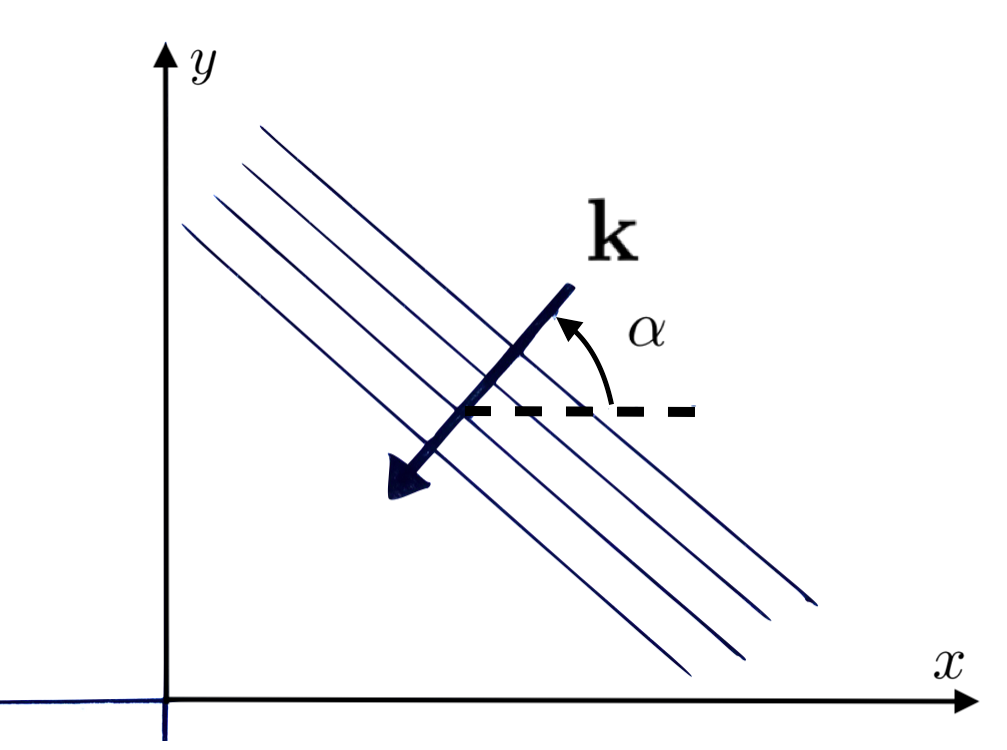
\includegraphics[width=6cm]{../figures/sk_incident_wave_2.png}
  \caption{Incident wave with wave vector $\vec{k}$}
  \label{fig:incident_wave}
\end{figure}

Finally, we introduce another potential, $\Phi$ which is a function of the spatial variables only. It will be useful to treat this potential by itself, since we already have an expression for the time dependence.

We will define
  \[\phi (x, y, z, t) = \Re[ \Phi(x,y,z)e^{-i\omega t} ]. \]

Then,
\begin{align*}
  \Phi e^{-i\omega t}
  &= (\Phi_r+i\Phi_i) (\cos(\omega t) - i\sin(\omega t)) \\
  &= \Phi_r \cos(\omega t)
      - i \Phi_r \sin(\omega t)
      + i \Phi_i \cos(\omega t)
      - (i)^2 \Phi_i \sin(\omega t)\\
  \therefore~ \Re[\Phi e^{-i\omega t}]
  &= \Phi_r \cos(\omega t) + \Phi_i \sin(\omega t)
\end{align*}
So then $\phi$ solves the time dependent linear wave equation. Finally, we want to show that for $\phi$ to solve the Helmholtz equation, $\Phi$ must solve it. This means we only need to find an expression for $\Phi$ to have an expression for the velocity field
\[\vec{u} = \nabla \phi = \nabla \Re[ \Phi(x,y,z)e^{-i\omega t} ].\]

\begin{propn} The potential $\phi$ solves the Helmholtz equation iff $\Phi$ solves the Helmholtz equation.
\end{propn}
\begin{proof}
\begin{align*}
  \nabla^2 \phi &= \frac{1}{c^2} \partialfrac{^2 \phi}{t} \\
  \Leftrightarrow \Re[ \nabla^2 \Phi(x,y,z)e^{-i\omega t} ]
  &= \Re \left[ \frac{1}{c^2} \partialfrac{^2 }{t} (\Phi(x,y,z)e^{-i\omega t}) \right]
\end{align*}
\begin{align*}
  \Re \left[
  \nabla^2 \Phi e^{-i\omega t}
  - \frac{1}{c^2}(-\omega^2) \Phi e^{-i\omega t}
  \right] &= 0 \\
  \Re \left[
  e^{-i\omega t} (\nabla^2\Phi + k^2\Phi)
  \right] &= 0.
\end{align*}
Since this must hold for all $t$,
\begin{equation*}
  \nabla^2 \Phi +k^2 \Phi = 0
\end{equation*}
as required.
\end{proof}
